\section{Prediction of Clinical Outcomes}
\label{sec:outcome}

In this section, we describe our modeling approaches and evaluation results to predict clinical outcomes using CT data, and using CT and clinical data.


%Our final model accuracy is 72\% (Using CT data + Clinical data), 39\% (using only CT data) at +/-3 years for ‘D from ct’. We will describe the model accuracy measurement method, improve model accuracy method, and the results for when using only CT data and when using CT data and clinical data.

\subsection{Modeling Approaches (CT data)}
\label{sec:model_ct}

We develop our approach in three steps, using a simple regression, using regressions with balanced training data, and using regressions after classifying the data into groups with balanced training data.
For each approach, we incrementally add features.


\begin{table}[!h]
    \centering
    \caption{Prediction accuracy for clinical outcomes}
    \begin{tabular}{l||c|c|c}
        \toprule[0.8pt]
         \textbf{Models} & \textbf{Test with dead} & \textbf{Test with alive} & \textbf{50\% mixed} \\\hline
         Regression                     & 5.33\% & 46.69\% & 26.01\% \\
         Balanced training data     & 32.0\% & 20.14\% & 26.07\% \\
         Classification and regression & 37.5\% & 40.51\% & 39.1\%\\
        \bottomrule[0.8pt]
    \end{tabular}
    \label{tab:clinical}
\end{table}


Table~\ref{tab:clinical} summarizes the prediction accuracy for clinical outcomes for our three approaches with different test sets.
We use 75\% of data for training and the rest for validation.
For the validation, we consider a prediction is correct if the difference of prediction and given response is within 3 years.
We note that we only show the results with the best learning models, i.e., neural network, due to limited space~\footnote{All the implemented models covering various classifiers and regressors are provided in our source codes}.

\begin{table}[!h]
    \centering
    \caption{Prediction accuracy of regressions}
    \begin{tabular}{l||c|c|c}
        \toprule[0.8pt]
         \textbf{Models} & \textbf{Test with dead} & \textbf{Test with alive} & \textbf{50\% mixed} \\\hline
    Linear regression & 5.33\% & 44.53\% & 24.93\% \\
    KNN regression & 1.33\% & 45.94\% & 23.64\% \\
    Neural network & 5.33\% & 46.69\% & 26.01\%\\
        \bottomrule[0.8pt]
    \end{tabular}
    \label{tab:reg}
\end{table}

\subsubsection{Regression}
We first use three regression models to predict clinical outcome, LinearRegression, KNeighborsRegressor (KNN), and MLPRegressor (Neural Network) from scikit-learn.
Table~\ref{tab:reg} shows the accuracy for each regression.
While all the regressions show relatively high accuracy, they report poor performance when testing with dead data, i.e., a testset that only consists of values given in column Death d from CT.
This is because only 5\% of our total dataset (494/8,887) are the dead data.
As the opposite case dominates, the model makes highly skewed predictions to the alive data.

%We use Linear regression, KNN regression, and Neural network to predict clinical outcome. Neural network accuracy has the highest accuracy of 26\%
%표 자리
%Problem:  The biggest problem with the above table results is low for Only dead group test result. This is because that 5\% (494/8,877) of our data set is given exact dead data. So, our model is skewed for Only alive group which we estimate dead data by Life expectation table. 


\subsubsection{Balanced training data}
To resolve the skew problem, we balance the ratio of dead and alive data in training data.
Table~\ref{tab:clinical} shows the performance improvement from the previous to current approach.
A balanced mix of the dead and alive data in training data improves the accuracy with dead test data, efficiently resolving the data skew, while that with alive test data decreases.

%Solving the above problem, we increased the ratio of people with a dead data in train set to 50\%. After that, we measured the result by dividing the case were death data and not. Every model, Linear regression, KNN regression, Neural network model, accuracy slightly increased by about 0.1\%. However, the prediction for the given case of death greatly improved from 5\% to 32\%. So, we can tell skewed problem is somewhat solved.

\begin{figure}[!h]
    \centering
    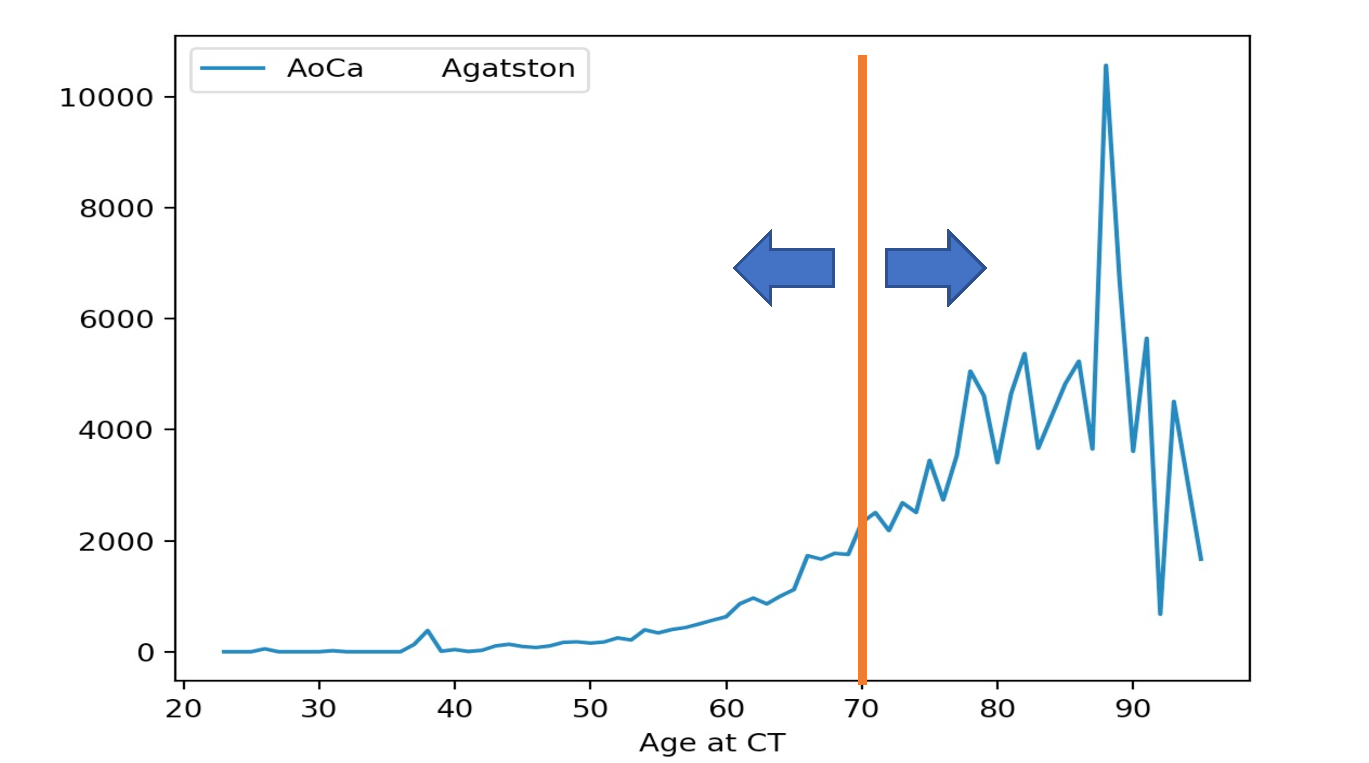
\includegraphics[width=0.65\textwidth]{figures/discrepancy.pdf}
    \caption{Data discrepancy in age distribution}
    \label{fig:discrepancy}
\end{figure}

\subsubsection{Classification and Regressions}
%그림 자리
We further analyze the data based on the distribution of age, and found out there is discrepancy between different ages, as shown in Figure~\ref{fig:discrepancy}.
That is, the value of AoCA Agaston increases in proportion to Age at CT within 70, but the observed values after then fluctuate, creating an irregular pattern.

To minimize the effect of the discrepancy, we classify the data into two groups, young and old, and run regression for each group.
We study our classification results in Section~\ref{sec:classification}.
Table~\ref{tab:clinical} reports the performance improvements between the previous and current increment.
Not only the accuracy with dead test data increases, but also that with alive test data improves by a large margin.

%We analyzed the data to improve the accuracy of the model and found that relation between age and CT data can be more explained, when we divide age into several groups. For example, in the case of AoCa Agaston, it increased in proportion to age until age 70, but had an irregular pattern from age 75. Furthermore, our classification model can distinguish someone is more than 70 or not with 85\% accuracy. So, if we divide the old and young groups using CT data and apply each regression model, we can have much higher accuracy. In fact, the accuracy improved by 15\% on average for each model.


\begin{table}[!h]
    \centering
    \caption{Prediction accuracy of classifications}
    \begin{tabular}{l||c|c|c}
        \toprule[0.8pt]
         \textbf{Models} & \textbf{Test with dead} & \textbf{Test with alive} & \textbf{50\% mixed} \\\hline
         Classification             & 16.22\% & 93.69\% & 54.96\% \\
         Balanced training data  & 64.83\% & 84.23\% & 74.53\% \\
         Augmented data          & 65.48\% & 85.81\% & 75.65\%\\
        \bottomrule[0.8pt]
    \end{tabular}
    \label{tab:classification}
\end{table}


\subsubsection{Classification}
\label{sec:classification}
We apply the same approach for classification as regressions stated above.
Table~\ref{tab:classification} shows the performance of stand-alone classification, classification with balanced training data, and augmented data (synthetically replicating dead data).
It follows the same performance trend as observed in the Section~\ref{sec:model_ct}.
Balanced ratio of the dead and alive data improves the accuracy for dead test data, and data augmentation further increases the performance of both tests.
We note that we use KNeighborsClassifier (KNN), GaussianNB (Naive Bayes), SGDClassifier (SVM), and MLPClassifier (Neural Network) in scikit-learn as our classifier models, but we only provide the results with MLPClassifier as using different classifiers only has small impact on the accuracy.
%We proceeded with the above- mentioned methods to improve the classification model of over 70 years or not. In addition, we proceeded data augment method. By adding over 80 years of age people more with simple transformation into the case of older group, we can improve classification model accuracy (from 74\% to 76\%)


\begin{figure}[!h]
    \centering
    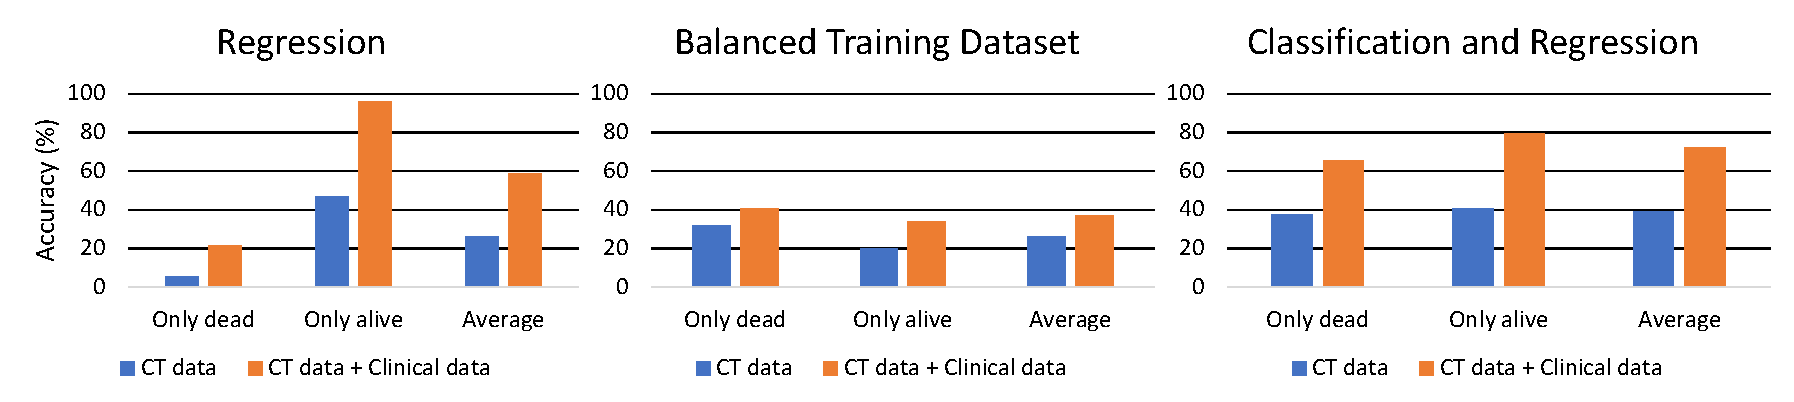
\includegraphics[width=0.95\textwidth]{figures/clinical.pdf}
    \caption{Accuracy comparisons with models using CT data, and models using both CT and clinical data}
    \label{fig:clinical}
\end{figure}

\subsection{Model Extension: using both Clinical and CT data}
\label{sec:clinical_CT}

We now apply our modeling approaches to further analyze the performance impact when clinical data are given.
Figure~\ref{fig:clinical} shows the accuracy comparisons between the models that use CT data, and the models that use both CT and clinical data for each approach.
The performance of those models using both CT and clinical data dominate that using CT data in every test case.

\begin{figure}[!h]
    \centering
    \begin{subfigure}{.48\textwidth}
        \centering
        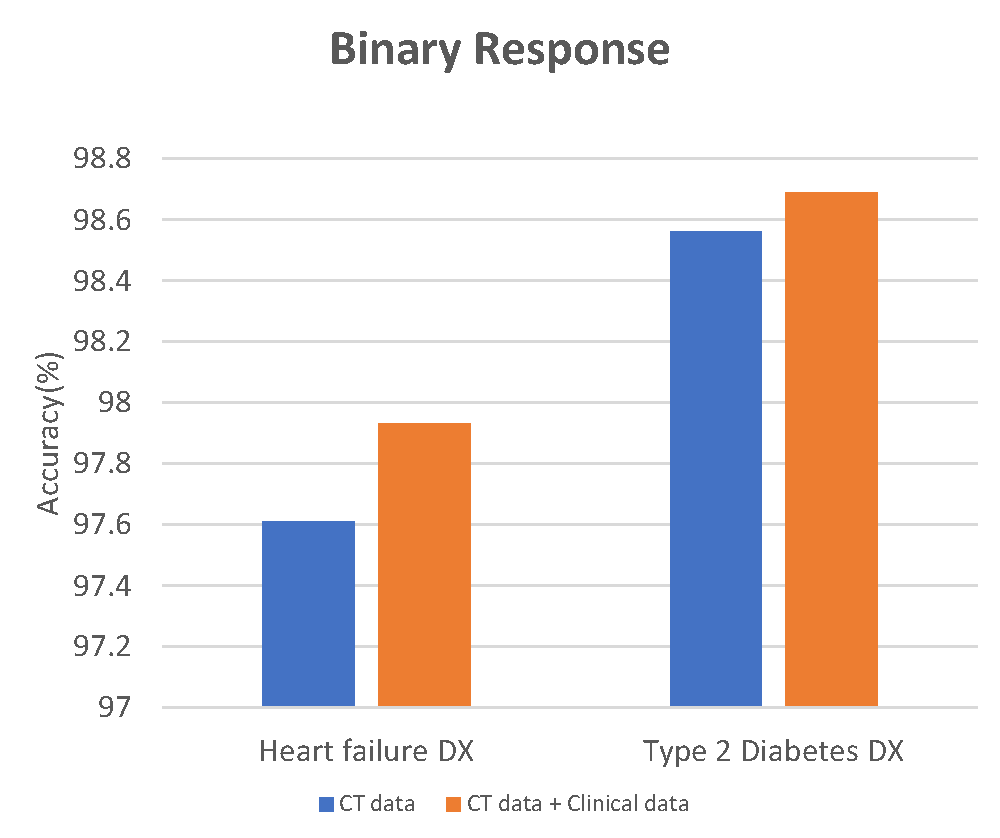
\includegraphics[width=.9\textwidth]{figures/binary_graph.pdf}
        \caption{Binary response}
        \label{fig:binary_outcome}
    \end{subfigure}
    \begin{subfigure}{.48\textwidth}
        \centering
        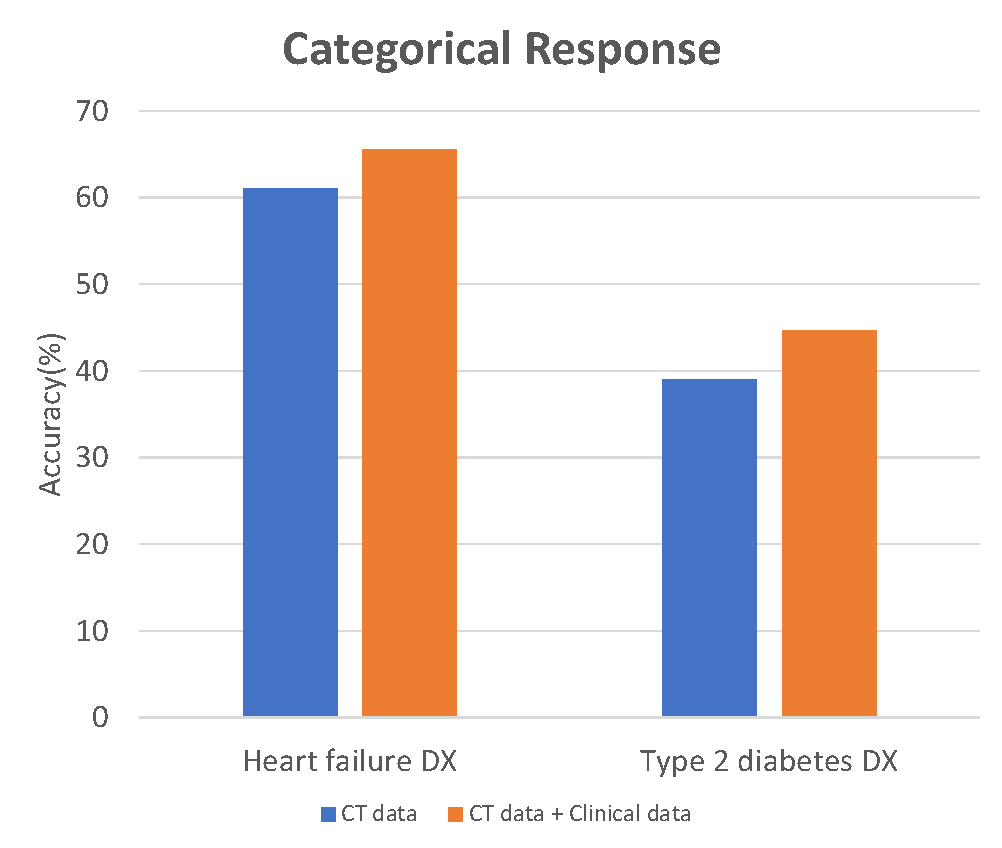
\includegraphics[width=.9\textwidth]{figures/categorical_graph.pdf}
        \caption{Categorical response}
        \label{fig:categorical_outcome}
    \end{subfigure}
    \caption{Accuracy comparisons with models using CT data, and models using both CT and clinical data for Heart Failure DX and Type 2 Diabetes DX prediction}
    \label{fig:clinical_outcome}
\end{figure}

\subsection{Model Extension: additional clinical outcomes}

Now we further dive into predicting additional clinical outcomes other than Death $[$d from CT$]$.
We use KNeighborsRegressor to predict a binary response, and a categorical response for Heart Failure DX and Type 2 Diabetes, as shown in Figure~\ref{fig:clinical_outcome}(a) and (b), respectively.
We note that the accuracy in each Figure is in a relative values, not fixing the range from 0 to 100\%.
From the results, we can infer that both the two models can efficiently predict Heart Failure DX and Type 2 Diabetes DX.
It is noteworthy that the accuracy improvement from the model using CT data to the model using both CT and clinical data is not as large as that observed in Section~\ref{sec:clinical_CT}.

%We predict Heart failure, Diabetes as additional clinical outcomes. KNN-regression(neighbor =10) has the best performance for this prediction and the detailed results are shown in the table below. The case using both CT data and clinical data shows 2.62\%(76.69\%,74.07\%) higher accuracy than the case where using only CT data. Especially,  when we predict 10 types of diabetes-DX messages and 27 types of heart failure-DX messages, using additional clinical data has a 5\% higher accuracy.

